\section{Methods and Materials}
% Here you should describe the design of your solution, your
% technical decisions, and why you believe your solution is appropriate. Some general
% images are recommended to enhance your explanation, and this section is expected
% to be 1 to 2 pages long. It is not recommended to include code here, but if you are
% presenting a complex algorithm, you may add it. Remember to write full paragraphs,
% with one idea per paragraph, and avoid using itemized lists. Aim for clarity and
% readability.


We began by drawing a component diagram to show how each part of our system fits together (see Fig. \ref{fig:component_diagram}). This diagram clarifies the relationships between our sensor inputs, the learning agent, and the robot’s control outputs before describing the technical details.

\begin{figure}[h]
    \centering
    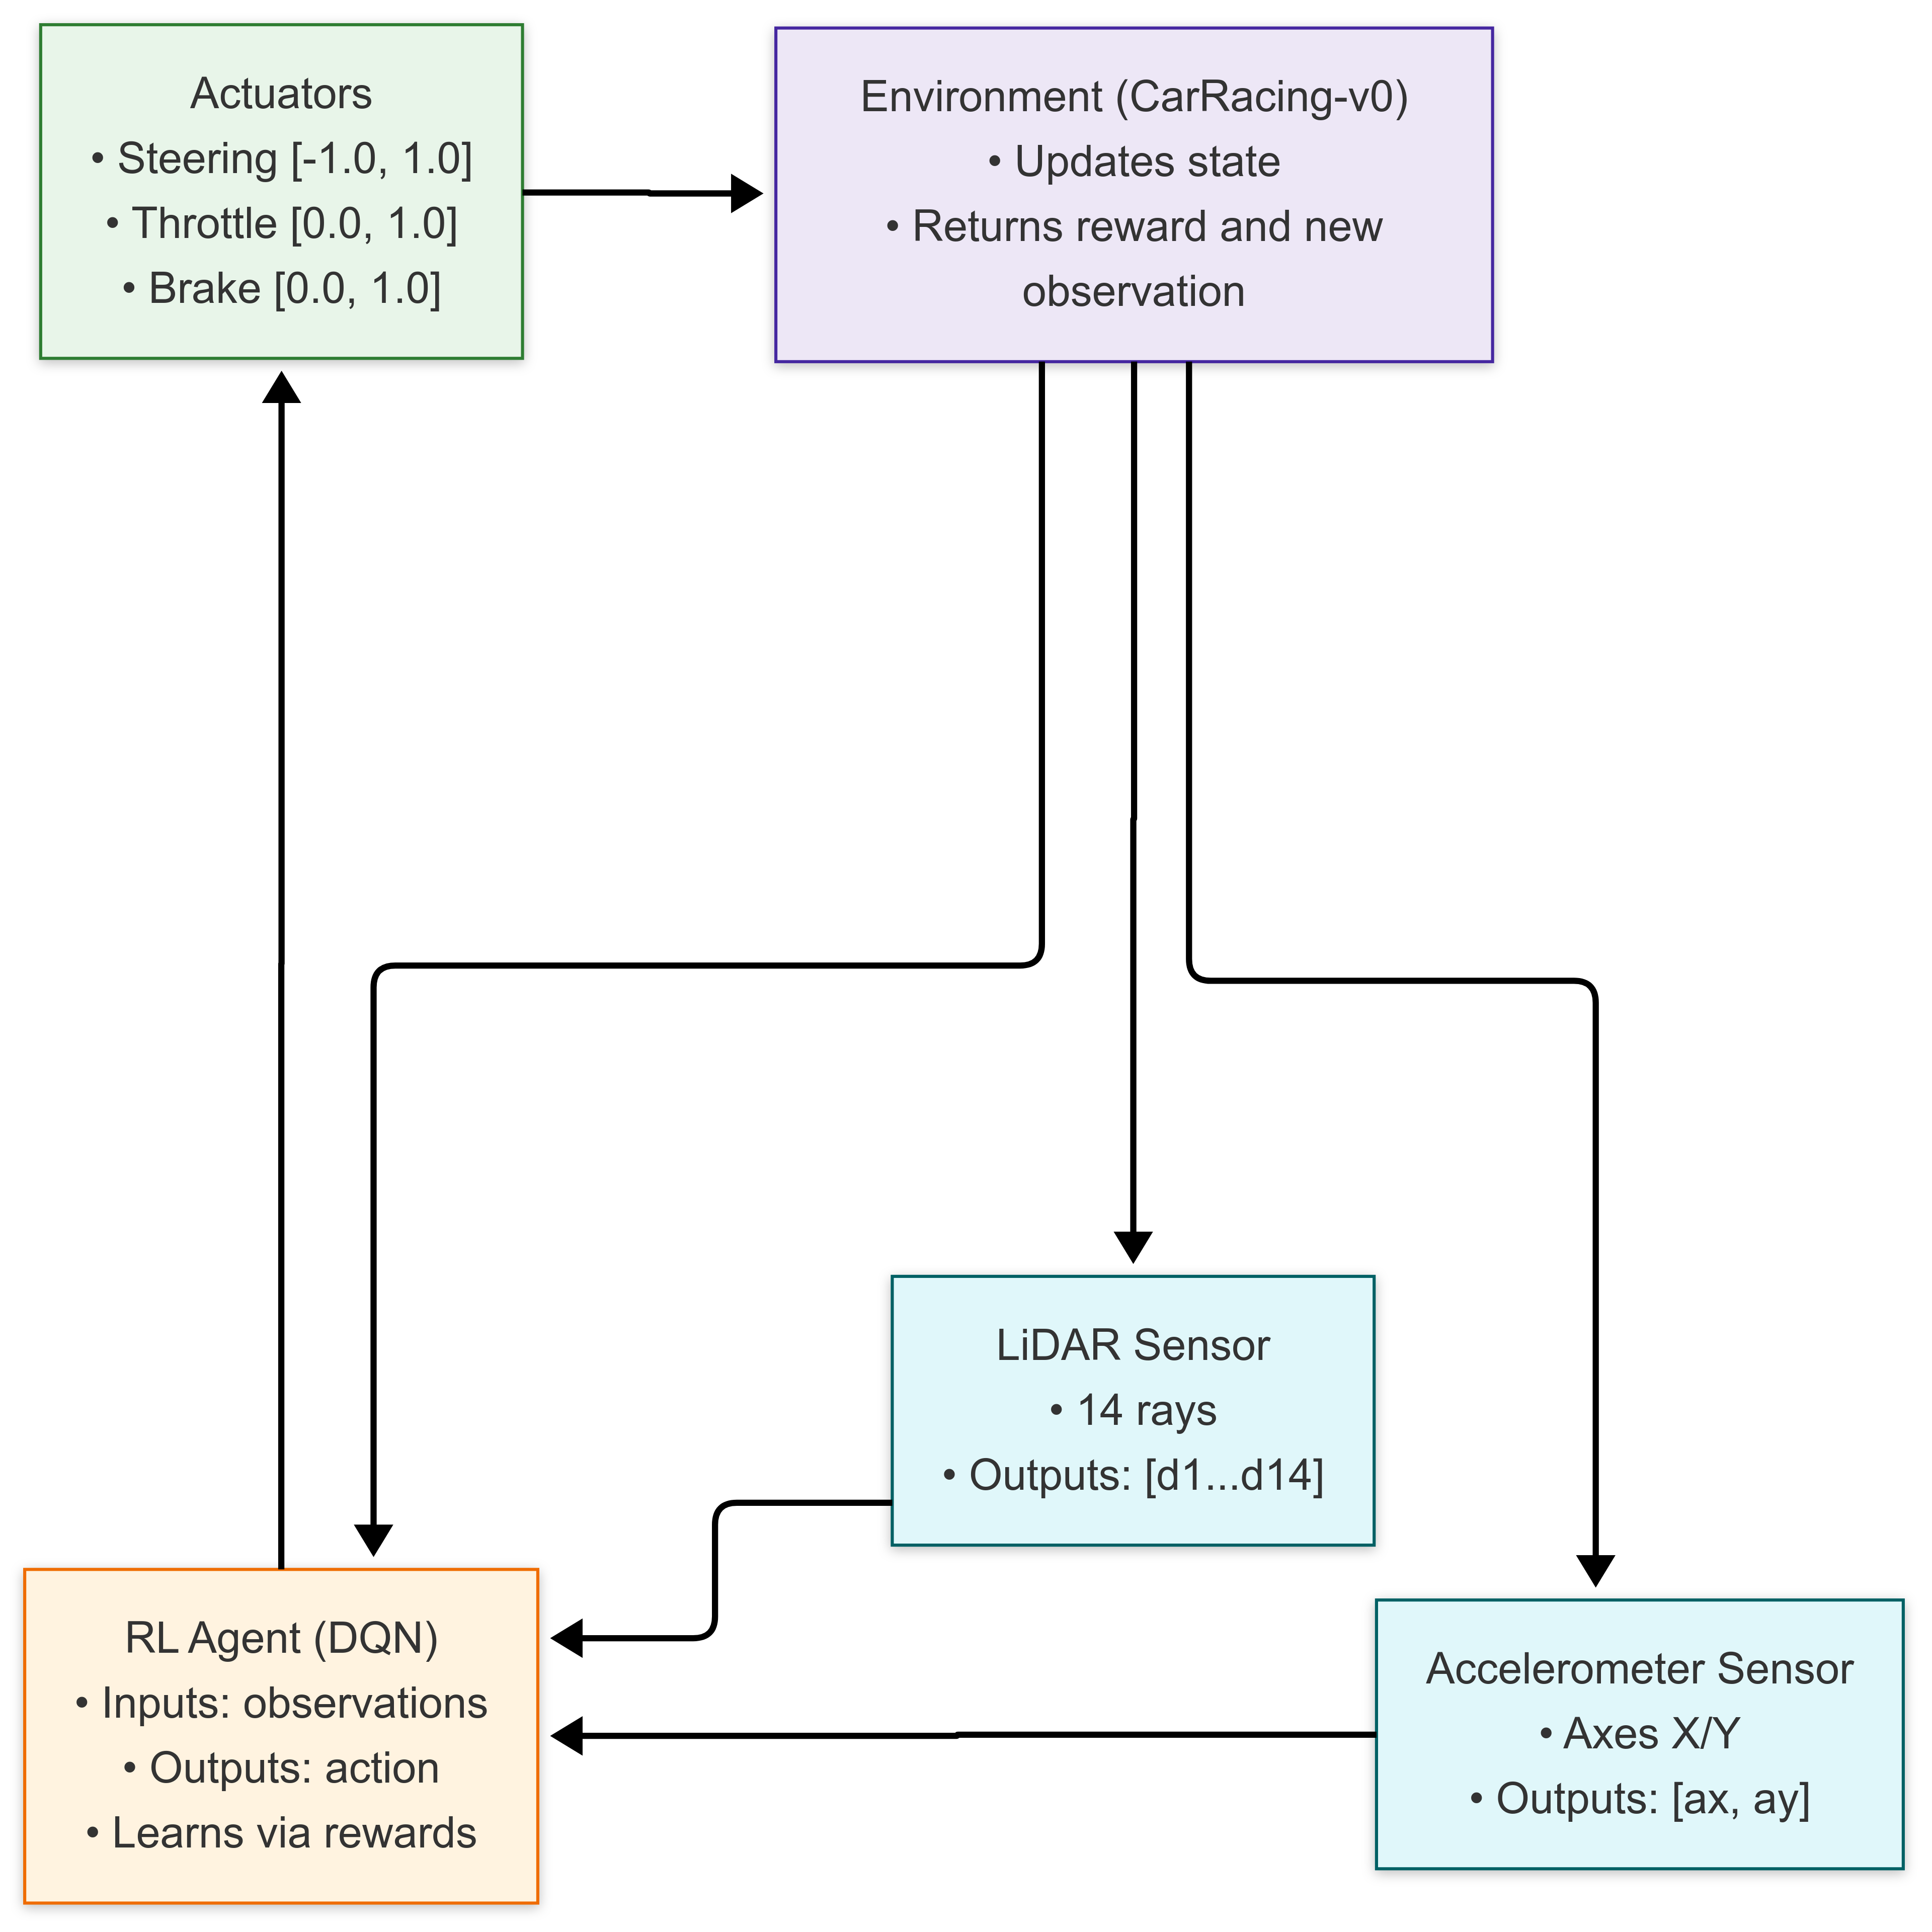
\includegraphics[width=0.8\linewidth]{images/ComponentDiagram.png}
    \caption{Component diagram of the system.}
    \label{fig:component_diagram}
\end{figure}

Our setup uses the CarRacing-v0 environment from Gymnasium, which provides a two-dimensional, top-down view of a procedurally generated racetrack. At each time step, the agent receives a single 96×96 RGB image showing the car at the center of the track. In addition to this visual input, Gymnasium exposes four ABS sensor readings (one for each wheel), true speed, steering position, and gyroscope measurements. We combine these data into a single state representation that the agent observes.

In addition to the visual and sensor data provided by the CarRacing-v0 environment, the initial problem formulation also considered the use of LiDAR sensors. We aim to explore the integration of LiDAR, potentially by modifying the existing environment or interfacing with a simulated LiDAR. This additional sensory input can be seamlessly incorporated into the state representation fed to our DQN agent, further enriching its perception of the surroundings.

To navigate and avoid obstacles, we implemented a Deep Q-Network (DQN) agent. The DQN uses a convolutional neural network to approximate the action-value function over continuous control actions—steering, gas, and brake. During training, the agent’s experiences (state, action, reward, next state) are stored in a replay buffer. We periodically sample mini-batches from this buffer to update the main network, while a separate target network—updated every few episodes—helps stabilize learning.

The reward function, provided by the Gymnasium CarRacing-v0 environment  \cite{gymnasium2023}, is designed to encourage both speed and track coverage. At each frame, the agent receives a \(-0.1\) penalty, which pushes it to finish the track quickly. Each newly visited track tile yields a bonus of \(1000/N\) points, where \(N\) is the total number of tiles. For example, covering all tiles in 732 frames yields:
\[
    1000 - 0.1 \times 732 \approx 926.8 \text{ points}.
\]
Crashing off-track for too long or failing to visit new tiles ends the episode.

\begin{figure}[h]
    \centering
    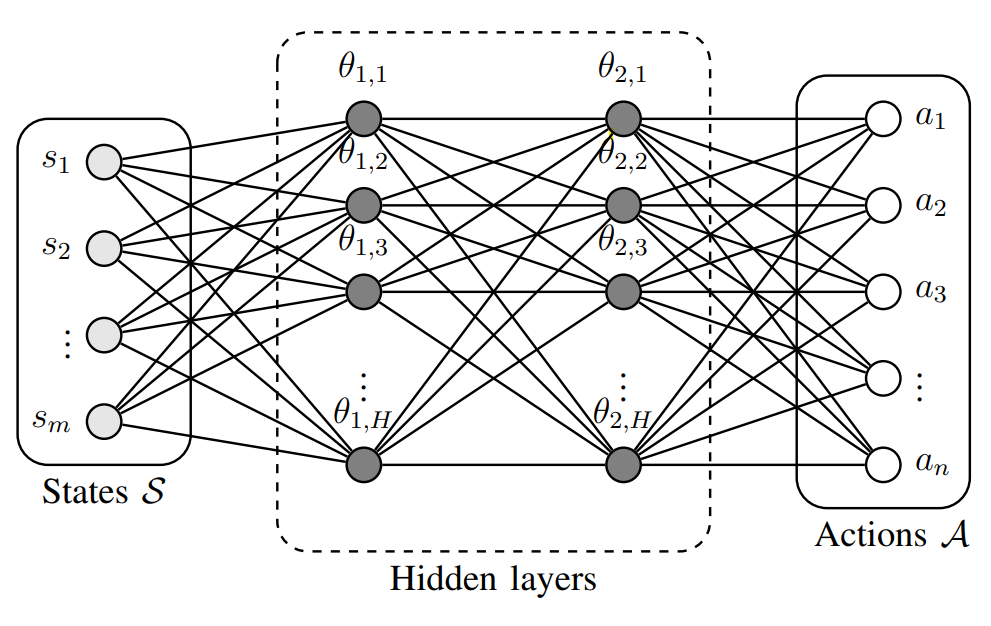
\includegraphics[width=0.8\linewidth]{images/DQNmodel.png}
    \caption{DQN algorithm diagram \cite{DQNimage}.}
    \label{fig:dqn_diagram}
\end{figure}

Figure \ref{fig:dqn_diagram} illustrates the overall DQN workflow. In our implementation, the input image and sensor readings pass through convolutional and fully connected layers to produce Q-values for each action. The action with the highest Q-value is selected at each step. Over thousands of episodes, the agent learns to balance acceleration, braking, and steering to maximize cumulative reward while avoiding track boundaries.

By combining visual information with sensor data and training with the DQN algorithm in the 2-D CarRacing-v0 environment, our system learns to navigate complex tracks efficiently and safely. This approach lays the foundation for future extensions, such as adding more sophisticated perception modules or testing on physical robots.

